\documentclass[11pt]{article}
\usepackage{amsmath}
%Gummi|065|=)
\title{\textbf{Finding adu distributions or finding photons}}
\author{Andrew Morgan}
\date{}
\usepackage{graphicx}
\begin{document}

\maketitle

\section{Maximum Likelihood for a single random variable}
Thought experiment:

\begin{itemize}

  \item We have a single discrete random variable x with a distribution $f(x)$
  \item $x$ is measured $N$ times but with an offset $f(x - \mu)$
  \item This is repeated $M$ times with $M$ different offsets
  \item $h^m_i$ is the histogram of $x_m$, the values of x on the m'th pixel, for $x_m = i$ in $0 \rightarrow I-1$

\end{itemize}


The probability of measuring our sequence of values $ x^m_n $ is:
\begin{align}
   Pr(x^m_n; f) &= \Pi_m^M \Pi_n^N f(x^m_n - \mu_m) = \Pi_m^M \Pi_i^I f(i - \mu_m)^{h^m_i}
\end{align}

The log likelihood is:
\begin{align}
   \ln(Pr(x^m_n; f)) &= \sum_m^M \sum_i^I h^m_i \ln(f(i - \mu_m))
\end{align}

Our log likelihood error is:
\begin{align}
   \varepsilon(\mu_n, f_i) &= -\sum_m^M \sum_i^I h^m_i \ln(f(i - \mu_m))
\end{align}
with a minimum value of 0. 


\begin{verbatim}

def log_likelihood_calc(f, mus, hists, prob_tol = 0.0):
    """
    Calculate the log likelihood error given a probability distribution f,
    a set of shifts mus, the measured histograms for each shift hists.
    
    log likelihood error = - sum_m sum_I hists[m, I] * ln( f[i-mus[m]] )
        
    As the pixel shifts need not be integer f[i-mus[m]] is calculated
    using the Fourier shift theorem and uses the function roll_real.
    
    Parameters
    ----------
    f : float array
        Real space values of f of length I.
    mus : float array
        The value in pixels of the shift amount of length M.
    hists : 2 dimensional integer array
        The measured values sampled from f shifted by the mus.
        hists must have the shape (M, I).
    prob_tol : float, optional
        Amount to add to f to aviod -infinity in the natural logarithm.
            
    Returns
    -------
    log_likelihood_error : float
        The log likelihood error.
    """
    error = 0.0
    for m in range(len(hists)):
        # only look at adu or pixel values that were detected on this pixel
        Is = np.where(hists[m] > 0)
        
        # evaluate the shifted probability function
        fs = roll_real(f, mus[m])[Is] 

        # sum the log liklihood errors for this pixel
        e  = hists[m, Is] * np.log(prob_tol + fs)
        error += np.sum(e)
    return -error


\end{verbatim}

\subsection{$\mu$ The offset's or dark values}
We could demand that the $\mu$'s are integer, so that shifting $f(i)$ is well defined. But this leads to problems in the minimization, since most refinement algorithms like a continuous set of variables and a continuous error function. Also we would expect that the shift of the distribution (or ``dark value") at a pixel may not be an integer multiple of counts. 

Another issue is that adding a constant to the mu's also corresponds to an overall shift in the probability distributions: $\mu + c \longleftrightarrow  f(i - c)$. We can remove this redundancy by demanding that the sum of the mu's is equal to 0. This can be automatically satisfied if we express the independent variables in Fourier space. Moving to Fourier space we have:

\begin{align} 
   \mu_m &= \frac{1}{M} \sum_{l=0}^{M-1} \hat{\mu}_l e^{2\pi i \frac{m l}{M}}, \\
   &= \frac{1}{M} \sum_{f_l=-M/2 + 1}^{M/2} \hat{\mu}_{f_l} e^{2\pi i mw_l} 
\end{align}

Since $\mu$ is real the reciprocal space representation has Hermitian symmetry. That is, the negative Fourier frequencies are the complex conjugate of the positive Fourier frequencies. In the discrete Fourier transform one can interpret the first element as the zero frequency of $\mu$(which is useful because we can demand that this is zero), the first half of the array as the positive frequencies and the second half of the array as the negative frequencies. Because of this it is useful switch between the array index, $m$ in this case, and the Fourier index, $f_l$. Thankfully Python already has a function for doing this:

\begin{verbatim}
 l   0  1  2  3  4  5  6  7    range(M)
 fl  0  1  2  3  4 -3 -2 -1    np.fft.fftfreq(M, d=1/float(M))
 wl (0  1  2  3  4 -3 -2 -1)/M np.fft.fftfreq(M)
\end{verbatim}

So now, our independent values for $\mu$ are:
\begin{align}
   \hat{\mu}_l \text{  for } l &= 1, 2, 3 .. M/2 + 1 \text{  where}\\
   \hat{\mu}_0 &= 0 \text{  and} \\
   \hat{\mu}_{l_f} &= \hat{\mu}^*_{-l_f}
\end{align}

\newpage
Let's make a function that returns the real-space real function corresponding to the Fourier components givin by Eq. (6).
\begin{verbatim}

def make_f_real(fhats, f_norm = 0.0):
    """
    Compute the real space representation of f given that 
    f is real and that sum_i f_i = f_norm. The fhats are 
    the complex Fourier space values of f from 1 to 
    N // 2 + 1 where N is the size of the real space array.
    
    Parameters
    ----------
    fhats : 1d complex array
        Fourier space values of f.
    f_norm : float, optional
        Sum of the real space function.
              
    Returns
    -------
    f : 1d float array
        the realspace representation of fhats given f_norm.
    """
    fh = np.concatenate( ([f_norm], fhats) )
    f  = np.fft.irfft(fh)
    return f
    
\end{verbatim}

The probability function f must also be normalized, but to 1. So it to should expressed in Fourier space. Now we must define how the shift will happen. Using the Fourier shift theorem we have:

\begin{align}
f_{i - \mu_m} = \frac{1}{I} \sum_{j=0}^{I-1} (\hat{f}_j e^{-2\pi i \mu_m w_j}) e^{2\pi i i w_j}
\end{align}

\begin{verbatim}

def shift_f_real(f, shift):
    """
    Apply the Fourier shift algorithm to f by shift pixels.
    
    Parameters
    ----------
    f : float array
        Real space values of f.
    shift : float
        The value in pixels of the shift amount.
            
    Returns
    -------
    f_shift : 1d float array
        The shifted representation of f.
    """
    fh      = np.fft.rfft(f)
    ramp    = np.exp(-2.0J * np.pi * shift * np.arange(float(fh.shape[0])) \
                     / float(f.shape[0]))
    f_shift = np.fft.irfft(fh * ramp)
    return f_shift

\end{verbatim}

Now we know have to define the independent variables for the probability (or adu) distribution $f$, the shift variables (or dark values) $\mu$. We can also calculate the real space values and shift the probability function. 

If we want to refine the set of $\mu$ values using a gradient based method then we must calculate the gradients. We need to find the vector gradient of the log likelihood error with respect to the independent $\mu$-variables. 

This is going to get messy... Let us try to evaluate the derivative with respect to the real part of the positive Fourier components of $\mu$ ($\hat{\mu}^r$). First we go down the derivative rabbit hole, then we climb our way back up: 

\begin{align}
   \frac{\partial \varepsilon(\mu, f)}{\partial \hat{\mu}^r_n} &= \frac{\partial}{\partial \hat{\mu}^r_n}\left[-\sum_m^M \sum_i^I h^m_i \ln(f(i - \mu_m))\right] \\
   &=  -\sum_m^M \sum_i^I h^m_i \frac{\partial}{\partial \hat{\mu}^r_n} \ln(f(i - \mu_m)) \\
   &=  -\sum_m^M \sum_i^I \frac{h^m_i}{f(i - \mu_m)} \frac{\partial f(i - \mu_m)}{\partial \hat{\mu}^r_n}
\end{align}


Fine, now we need to evaluate the final term:
\begin{align}
   \frac{\partial f(i - \mu_m)}{\partial \hat{\mu}^r_n} &= \frac{\partial}{\partial \hat{\mu}^r_n} \frac{1}{I} \sum_{j=0}^{I-1} (\hat{f}_j e^{-2\pi i \mu_m w_j}) e^{2\pi i i w_j} \\
   &= \frac{1}{I} \sum_{j=0}^{I-1} (\hat{f}_j e^{-2\pi i \mu_m w_j}) e^{2\pi i i w_j} \left[-2\pi i w_j \frac{\partial \mu_m}{\partial \hat{\mu}^r_n} \right]
\end{align}


OK, and the last term again:
\begin{align}
   \frac{\partial \mu_m}{\partial \hat{\mu}^r_n} &= \frac{\partial}{\partial \hat{\mu}^r_n} \left[\frac{1}{M} \sum_{f_l=-M/2 + 1}^{M/2} \hat{\mu}^r e^{2\pi i mw_l} \right] \\ 
   &= \frac{1}{M} \sum_{f_l=-M/2 + 1}^{M/2} \frac{\partial \hat{\mu}^r_{f_l}}{\partial \hat{\mu}^r_n} e^{2\pi i mw_l} 
\end{align}


We have to be carefull here. Remember that $\hat{\mu}$ is Hermitian, so not all of the $\hat{\mu}^r$ are independent:
\begin{align}
   \frac{\partial \mu_m}{\partial \hat{\mu}^r_n} &= \frac{1}{M} \sum_{f_l=-M/2 + 1}^{-1} \delta_{f_n + f_l} e^{2\pi i mw_l} + \frac{1}{M} \sum_{f_l=1}^{M/2-1} \delta_{f_n - f_l} e^{2\pi i mw_l} \\
   &+ \frac{1}{M} \delta_{f_n - 0} + \frac{1}{M} \delta_{f_n - M/2} e^{\pi i m} \\
   &= \frac{1}{M} \sum_{f_l=1}^{M/2-1} \delta_{f_n - f_l} \left[e^{-2\pi i mw_n} + e^{2\pi i mw_n} \right] + \frac{1}{M} \delta_{f_n - 0} + \frac{1}{M} \delta_{f_n - M/2} (-1)^m\\
   &= \frac{2}{M} \cos(2\pi mw_n) \sum_{f_l=1}^{M/2-1} \delta_{f_n - f_l} + \frac{1}{M}\left(\delta_{f_n - 0} +  (-1)^m \delta_{f_n - M/2} \right)
\end{align}

Notice those two extra anoying bits on the right? Well we don't have to worry about $n = 0$ because are keeping the $\mu$ values normalised to 0, but that $(-1)^m$ comes about when the array dimensions are even. Hmmm... I guess we should keep M even for now but I am sure it cannot be that hard to work out the odd case. 

\pagebreak
While we are here I guess we should look at the derivative with respect to $\hat{\mu}^i$:
\begin{align}
   \frac{\partial \mu_m}{\partial \hat{\mu}^i_n} &= -\frac{i}{M} \sum_{f_l=-M/2 + 1}^{-1} \delta_{f_n + f_l} e^{2\pi i mw_l} + \frac{i}{M} \sum_{f_l=1}^{M/2-1} \delta_{f_n - f_l} e^{2\pi i mw_l} \\
   &= \frac{1}{M} \sum_{f_l=1}^{M/2-1} \delta_{f_n - f_l} \left[-ie^{-2\pi i mw_n} + ie^{2\pi i mw_n} \right] \\
   &= -\frac{2}{M} \sin(2\pi mw_n) \sum_{f_l=1}^{M/2-1} \delta_{f_n - f_l} 
\end{align}

We can bring the real and imaginary parts together:
\begin{align}
   \frac{\partial \mu_m}{\partial \hat{\mu}_n} &\equiv \frac{\partial \mu_m}{\partial \hat{\mu}^r_n} + i \frac{\partial \mu_m}{\partial \hat{\mu}^i_n} \\
   &= \frac{2}{M} \left[\cos(2\pi mw_n) - i\sin(2\pi mw_n)\right] \sum_{f_l=1}^{M/2-1} \delta_{f_n - f_l} \\
   &+ \frac{1}{M}\left(\delta_{f_n - 0} +  (-1)^m \delta_{f_n - M/2} \right) \\
   &= \frac{2}{M} e^{-2\pi i m w_n} \sum_{f_l=1}^{M/2-1} \delta_{f_n - f_l} + \frac{1}{M}\left(\delta_{f_n - 0} +  (-1)^m \delta_{f_n - M/2} \right)
\end{align}

As an aside, one can view the two dimensional matrix in Eq. (27) as a discrete cosine transformation matrix of the first kind http://docs.scipy.org/doc/scipy-0.15.1/reference/generated/scipy.fftpack.dct.html (after multiplying by M).

At this point we are at the bottom of the rabitt hole. And remember that it is easier to go down than up! 

Put Eq. (27) back into Eq. (14):
\begin{align}
   \frac{\partial f(i - \mu_m)}{\partial \hat{\mu}_n} &= \frac{1}{I} \sum_{j=0}^{I-1} (\hat{f}_j e^{-2\pi i \mu_m w_j}) e^{2\pi i i w_j} \left[-2\pi i w_j \frac{\partial \mu_m}{\partial \hat{\mu}_n} \right] \\
   &= \frac{\partial \mu_m}{\partial \hat{\mu}_n} \frac{1}{I} \sum_{j=0}^{I-1} (-2\pi i w_j \hat{f}_j e^{-2\pi i \mu_m w_j}) e^{2\pi i i w_j} 
\end{align}


There are three essensial parts to Eq. (22) first is the derivative term $\frac{\partial \mu_m}{\partial \hat{\mu}_n}$ which is a two dimensional function outside of the sum. The second is the multimplication (inside the sum) by $e^{-2\pi i \mu_m w_j}$ which as we already know has the effect of shifting $f$ in real space by $\mu_m$. The final part is the multiplication by $-2\pi i w_j$, in real space this is like taking the spatial derivative of $f$. As the second and third parts commute (they are both multiplications in Fourier space) I will define their effect with this notation:
\begin{align}
   f'_i &\equiv \frac{1}{I} \sum_{j=0}^{I-1} -2\pi i w_j \hat{f}_j e^{2\pi i i w_j} \\
   f'_{i-\mu_m} &\equiv \frac{1}{I} \sum_{j=0}^{I-1} (-2\pi i w_j \hat{f}_j e^{-2\pi i \mu_m w_j}) e^{2\pi i i w_j} 
\end{align}

\begin{verbatim}

def grad_shift_f_real(f, shift):
    """
    Apply the Fourier shift algorithm to f by shift pixels. 
    In addition take the gradient of f.
    
    Parameters
    ----------
    f : float array
        Real space values of f.
    shift : float
        The value in pixels of the shift amount.
            
    Returns
    -------
    f_shift : 1d float array
        The gradient of the shifted representation of f.
    """
    fh      = np.fft.rfft(f)
    lramp   = -2.0J * np.pi * np.arange(float(fh.shape[0])) \
              / float(f.shape[0])
    ramp    = lramp * np.exp(shift * lramp)
    f_shift = np.fft.irfft(fh * ramp)
    return f_shift

\end{verbatim}

\iffalse
\begin{figure}[htp]
\centering
\includegraphics[scale=0.50]{/home/amorgan/Physics/git_repos/MaxLhist/shifted_gradient.png}
\caption{Example of the shifted gradient of a gaussian. Using grad\_shift\_f\_real.}
\label{shifted_grad}
\end{figure}
\fi

With that done, I will use the notation from Eq. (31) to express the derivative of the probability function with respect to the real and imaginary components of the Fourier spectrum of the shift values:
\begin{align}
   \frac{\partial f(i - \mu_m)}{\partial \hat{\mu}_n} &=  \frac{\partial \mu_m}{\partial \hat{\mu}_n} \times f'_{i-\mu_m}
\end{align}


Now we can go back to Eq. (12):
\begin{align}
   \frac{\partial \varepsilon(\mu, f)}{\partial \hat{\mu}_n} &= -\sum_m^M \sum_i^I \frac{h^m_i}{f(i - \mu_m)} \frac{\partial \mu_m}{\partial \hat{\mu}_n} \times f'_{i-\mu_m} \\
   &= -\sum_m^M  \frac{\partial \mu_m}{\partial \hat{\mu}_n} \sum_i^I \frac{h^m_i}{f(i - \mu_m)} \times f'_{i-\mu_m}
   \label{mu_grad}
\end{align}


As it stands we have function of $i$ (the adu values) and $m$ (the pixel numbers) just before the sum over the adu values. Then we have a transform from $m\rightarrow n$, where the transform matrix is given by $\frac{\partial \mu_m}{\partial \hat{\mu}_n}$ which is independant of the model and the data. So what does this transform look like?
\begin{align}
   g_n &= \sum_{m=0}^{M-1} \left[ \frac{2}{M} e^{-2\pi i m w_n} \sum_{f_l=1}^{M/2-1} \delta_{f_n - f_l} + \frac{1}{M}\left(\delta_{f_n - 0} +  (-1)^m \delta_{f_n - M/2} \right) \right] \times h_m
\end{align}

This is rather strange, note that the transform sums over $m$ not $n$, so it does not reduce to the discrete cosine transform of the first kind. Regardless, 
\begin{align}
   g_n &= \frac{1}{M} \sum_{m=0}^{M-1} h_m                      &&\text{for } n = 0 \\
   &= \frac{2}{M} \sum_{m=0}^{M-1} e^{-2\pi i m w_n} \times h_m &&\text{for } 0 < n < \frac{M}{2} \\
   &= \frac{1}{M} \sum_{m=0}^{M-1} (-1)^m h_m                   &&\text{for } n = \frac{M}{2}
\end{align}

\pagebreak
\begin{verbatim}

def mu_transform(h):
    """
    Calculate a strange transform. So far only works
    when h.shape[0] is an even number (and h is 1D).
    Note that in the output n = 0 is excluded.
	
    g[n] = 1/M sum_m=0^M-1 h[m]                         for n = 0
    g[n] = 2/M sum_m=0^M-1 e^(-2 pi i m n / M) h[m]     for 0 < n < M/2
    g[n] = 1/M sum_m=0^M-1 (-1)^m h[m]                  for n = M/2
    
    Parameters
    ----------
    h : 1D float array
        Values of h of length M.
            
    Returns
    -------
    g : 1D complex array
        g for n = 1, ..., M/2, so with the shape M/2 
    """
    if h.shape[0] % 2 == 1 :
        raise ValueError('input array shape must even for now')
    g = np.zeros((h.shape[0] / 2, ), dtype = np.complex128)
    
    #g[0]     = np.sum(h) / float(M)
    g[1 : -1] = np.fft.fft(h)[1 : M/2] * 2. / float(M)
    g[-1]     = np.sum(h * (-1)**np.arange(h.shape[0]) ) / float(M)
    return g
\end{verbatim}





\subsection{example}
Let's see if this actually works. As an example we will start with a simple problem where the adu distribution is a gaussian, with a sigma of 5 adus centered on 100 adus:
\begin{align}
   f(i) &= \frac{1}{\sigma \sqrt{2\pi}} e^{- \frac{(x - \mu)^2}{2\sigma^2}} \\
        &= \frac{1}{5 \sqrt{2\pi}} e^{- \frac{(x - 100)^2}{2\times 25}}
\end{align}

Where $\mu$ in Eq. 39 is the mean of $f$ not the shift coordinates. The real space shift coordinates are (say) -20 and 20 adus (remember that their sum must be 0):
\begin{align}
   \mu       &= [\mu_0, \mu_1] = [-20, 20] \\
   \hat{\mu} &= [\hat{\mu_0}, \hat{\mu}_1] = [0 + 0i, -40 + 0i]
\end{align}
here we can see that, as expected, there is only one non-zero value (-40) which is our single unknown variable in this retrieval.

Now we do an experiment for (say) 1000 shots, our data looks like:
\begin{figure}[htp]
\centering
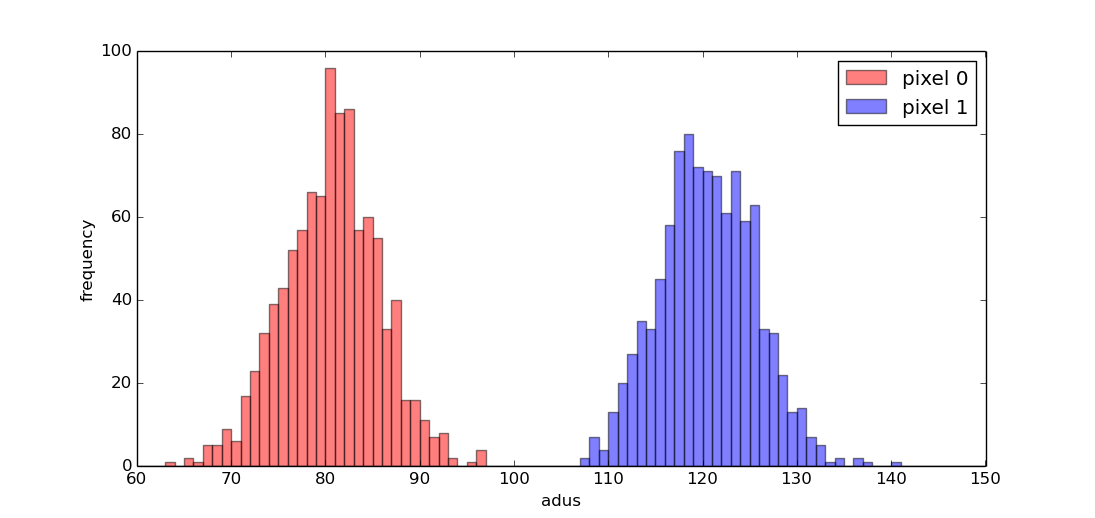
\includegraphics[scale=0.50]{figure_1.png}
\caption{adu histogram of two pixels}
\label{data}
\end{figure}

\begin{figure}[htp]
\centering
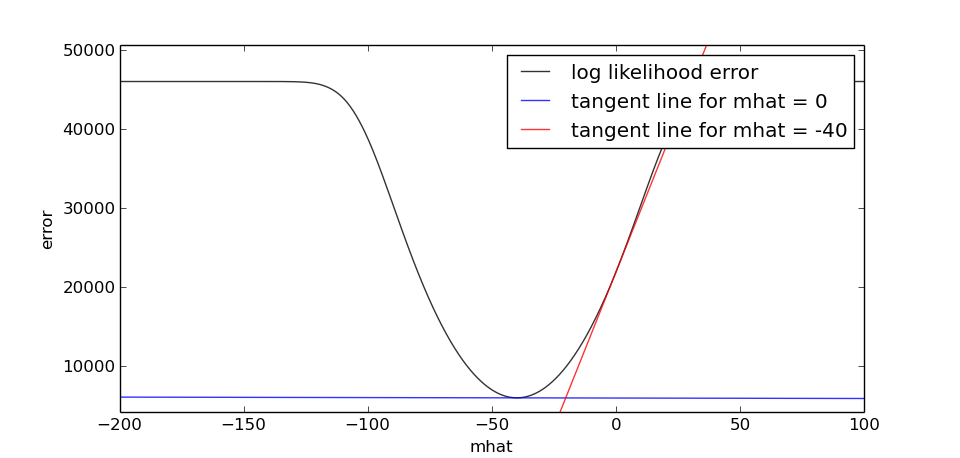
\includegraphics[scale=0.50]{figure_3.png}
\caption{log likelyhood error with a tolerance of $10^{-10}$.}
\label{error}
\end{figure}
Now let's look at the error as a function of $\hat{\mu}_1^r$ in Fig. \ref{error}. The good thing is that the error seems nice and quadratic near the correct value of $\hat{\mu}_1^r$ (-40) however we can also see that the error flattens out at larger or lower values. This is due to rounding errors in the natural logarithm, when evaluating the error metric. Basically, if our initial guess for the $\mu$ values is inside the flat region then we are screwed.

Also shown are the tangent lines for $\hat{\mu}^r_1 = 0$ and $-40$, calculated using Eq. (\ref{mu_grad}) which look resonable. Note that we do not expect the gradient at the correct solution (-40) to be zero, this is because we do not have perfect statistics of the function $f$ in the histograms.

So, starting at some value for $\hat{\mu}^0$, we would then like to find the local minimum (-40) of the log likelihood error. We will start with the simplest approach, and completely disregard computational efficiency for now. Starting at $\hat{\mu}^0$ we can compute the steepest descent direction $-\frac{\partial \varepsilon(\mu, f)}{\partial \hat{\mu}_n}|_{\hat{\mu}^0}$ then step along this line until we are close enough to the local minimum of the error to look for the next search direction. 

We have many options for the line search but let's start with something very simple (and very slow); the bisection method [google it]. 

\iffalse
But before we dive into this our lives will be much easier if we have a real set of variables and gradients. In the code below $\mu$, $\hat{\mu}$ and $\hat{\mu}_\text{extended}$ are all interchangable:

\begin{verbatim}

def mu_to_muextended(mu):
    """
    Converts the real vector mu into the real independent Fourier
    space variables, when the normalisation of mu is fixed and 
    mu.shape[0] is even. The first half + 1 are the real positive 
    Fourier components of mu while the second half - 1 are the
    imaginary positive Fourier components of mu.

    mu_extended = np.array([np.fft.rfft(mu).real[ 1 : ], \
                            np.fft.rfft(mu).imag[ 1 : -1])

    Parameters
    ----------
    mu : 1D float array
        Values of mu of length N.
            
    Returns
    -------
    mu_extended : 1D float array
        Values of the "independent" Fourier components of mu when the 
        normalisation of mu is fixed. Of length N - 1.
    """
    muhat       = np.fft.rfft(mu)
    mu_extended = np.concatenate((muhat.real[1 :], muhat.imag[1 : -1]))
    return mu_extended

def muextended_to_mu(mu_extended, norm = 0.0):
    """
    Inverse of mu_to_muextended

    Parameters
    ----------
    mu_extended : 1D float array
        Values of the "independent" Fourier components of mu when the 
        normalisation of mu is fixed. Of length N - 1.

    norm : float
        The normalisation of mu = np.sum(mu).
            
    Returns
    -------
    mu: 1D float array
        Values of mu of length N.
    """
    N                 = mu_extended.shape[0] + 1
    muhat             = np.empty( (N / 2 + 1,) , dtype=np.complex128)
    muhat[0]          = norm
    muhat[1 :]        = mu_extended[: N / 2]
    muhat[1 : -1].imag= mu_extended[N/2 : ]
    mu                = np.fft.irfft(muhat)
    return mu

\end{verbatim}
\fi

As we step along the steepest descent direction $d$, from the point $\hat{\mu}^0$ the gradient along this line is given by:
\begin{align}
   \varepsilon'(\alpha) &= \Re\left\{\sum_n \hat{d}^*_n \frac{\partial \varepsilon(\mu, f)}{\partial \hat{\mu}_n}|_{\hat{\mu}^0 + \alpha \hat{d}} \right\}
   \label{directional_derivative}
\end{align}
To find the minimum of $\varepsilon(\alpha) = \varepsilon(\mu^0 + \alpha d, f)$ we can then find the root of the Eq. \ref{directional_derivative}. 

\begin{figure}[htp]
\centering
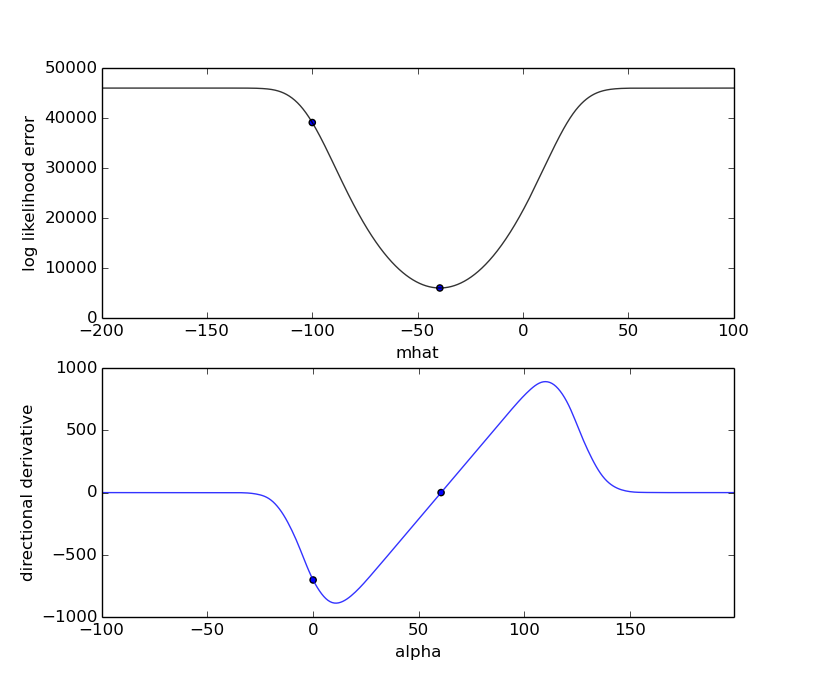
\includegraphics[scale=0.50]{figure_4.png}
\caption{log likelyhood error with a tolerance of $10^{-10}$ (top) showing the starting guess (-100) and the end position after the bisection minimisation (-40.21). The directional derivative, where $\hat{d}$ has been normalised.}
\label{bisection}
\end{figure}

The result of the bisection line search is shown in Fig. \ref{bisection}. 

\begin{verbatim}
def mu_bisection(f_alpha, min_step = 1.):
    # find a and b
    a = 0.0
    b = min_step
    fa = f_alpha(a)
    while fa * f_alpha(b) > 0 :
        b = 2 * b
    x0, r = scipy.optimize.bisect(f_alpha, a, b, xtol=1e-2, \
    rtol=4.4408920985006262e-16, maxiter=100, full_output=True, disp=True)
    return x0

def mu_directional_derivative(d, f, muhat, hists, prob_tol = 1.0e-10):
    jacobian = jacobian_mus_calc(f, muhat, hists, prob_tol = 1.0e-10)
    return np.sum((jacobian * np.conj(d)).real)

def jacobian_mus_calc(f, mushat, hists, prob_tol = 1.0e-10):
    mus = make_f_real(mushat)
    # this could be more efficient
    f_prime_shift = np.zeros_like(hists, dtype=np.float64)
    for m in range(len(mus)) :
        f_prime_shift[m] = grad_shift_f_real(f, mus[m]) \
        / (prob_tol + roll_real(f, mus[m]))
    
    temp  = hists * f_prime_shift 
    temp  = np.sum(temp, axis=1)
    mus_f = mu_transform(temp)
    return -mus_f

\end{verbatim}

And finally we use the same code to solve for a list of 10 $\mu$ values from 10 histograms, each with 50 counts. The results are shown in Fig. \ref{more_mus}.
\begin{figure}[htp]
\centering
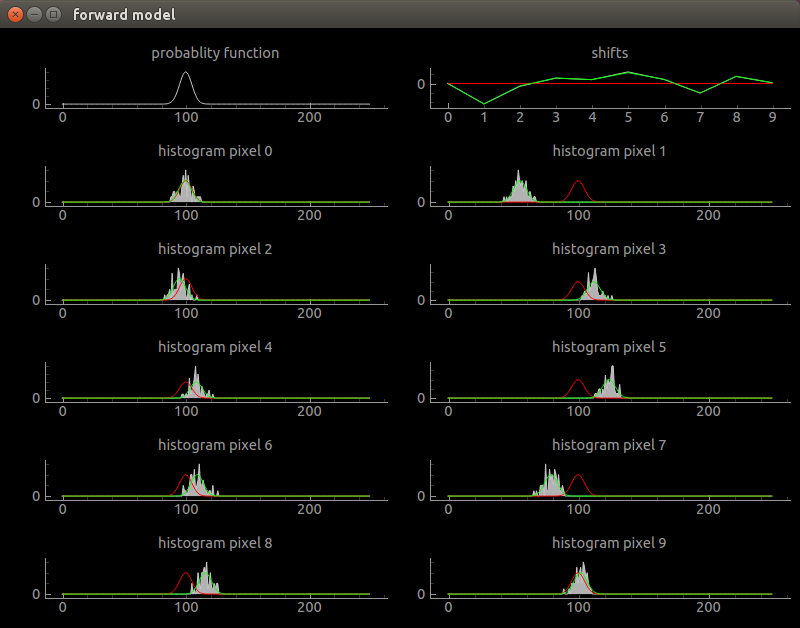
\includegraphics[scale=0.50]{figure_5.png}
\caption{Result of refining the initial estimate for the set of shift coordinates. The initial estimates are all zero (red lines) and the refined values are shown in green. The filled white plots are the histogram data. }
\label{more_mus}
\end{figure}

\subsection{Project a vector onto the set of vectors with sum = 0 and some elements = 0}
If we have a mask $M$ and (general) vector $v$ then the projection of $v$ onto the set of vectors for which $\sum v = 0$ and $M \cdot v = v$ is given by:
\begin{align}
   v'_n = P \cdot v = M_n \left[ v_n - \frac{\sum_m v_m M_m}{\sum_m M_m} \right]
\end{align}




\subsection{$f$ The probability (or adu) distribution}
Hopefully most of the infrastructure is already in place now to refine the values of $f$ given a set of $\mu$ values without too much pain.  
\begin{align}
   \frac{\partial \varepsilon(\mu, f)}{\partial f_j} &= -\frac{\partial}{\partial f_j} \sum_m^M \sum_i^I h^m_i \ln(f(i - \mu_m)) \\
   &= -\frac{\partial}{\partial f_j} \sum_m^M \sum_i^I h^m_{i+\mu_m} \ln(f_i) \\
   &= -\sum_m^M \sum_i^I h^m_{i+\mu_m} \frac{\delta_{i-j}}{f_i} \\
   &= -\frac{\sum_m^M h^m_{j+\mu_m}}{f_j}
\end{align}

In the present case this gradient vector will simply encourage ever increasing values of $f$. That is, we have to keep $f$ normalised. Now we could do this by representing $f$ in Fourier space and recalculating the gradient vector there (as we did for $\mu$). But then we also have the problem that values of $f$ for which $\sum_m^M h^m_{j+\mu_m}$ is zero have no effect on the error metric. Thus they are completely free to float in order to satisfy any normalisation constraint.

What we can do instead is simply project the gradient vector onto the closest vector that has a normalisation of zero, and is zero when $M_j (= \sum_m^M h^m_{j+\mu_m} > 0)$ is zero:
\begin{align}
   \nabla f_j &= P \cdot \frac{\partial \varepsilon(\mu, f)}{\partial f} \\
   &= -M_j \left[\frac{\sum_m^M h^m_{j+\mu_m}}{f_j}  - \frac{\sum_i M_i (\sum_m^M h^m_{i+\mu_m})/f_i}{\sum_i M_i} \right]
\end{align}

%\begin{align}
%   \nabla f_j &= P \cdot \frac{\partial \varepsilon(\mu, f)}{\partial f} \\
%   &= -\left[\frac{\sum_m^M h^m_{j+\mu_m}}{f_j}  - \frac{1}{I} \sum_i \frac{\sum_m^M h^m_{i+\mu_m}}{f_i} \right]
%\end{align}


\end{document}


